\chapter{Introducción}
\section{Aprendizaje automático semi-supervisado}

El aprendizaje automático es un campo de las ciencias de la computación que intenta dotar a los sistemas informáticos de la capacidad de aumentar
progresivamente su habilidad en una tarea específica, sin la necesidad de ser específicamente programados para tal tarea \citep{samuel1959some}. Dentro de este
campo podemos identificar dos grandes grupos de técnicas: las de aprendizaje supervisado y las de aprendizaje no supervisado. Las primeras utilizan un conjunto
de datos que traen asociados una etiqueta de clase (que indica a qué clase pertenece el objeto) o valor de salida deseado. El proceso de aprendizaje consiste en
generar un modelo que logre mapear los datos de entrada a los valores de salida deseados \citep{russell2016artificial}. El modelo además debe ser capaz de
generalizar, es decir, generar salidas correctas cuando reciba como entrada datos no vistos durante el proceso de aprendizaje. Por otro lado, en el aprendizaje
no supervisado el objetivo es generar modelos que descubran grupos o relaciones subyacentes en los datos sin utilizar ningún tipo de etiqueta o valor de salida
esperado.

Como punto intermedio entre los dos grupos de técnicas antes mencionados, apareció un nuevo grupo de algoritmos, llamados de aprendizaje
semi-supervisado \citep{chapelle2006semi}. Este tipo de algoritmos utiliza ejemplos etiquetados para aprender la distribución de las clases de la misma forma
que los métodos de aprendizaje supervisado, pero además aprovecha ejemplos no etiquetados para modelar mejor el espacio de las características y así mejorar las
tasas de clasificación. Como los ejemplos no etiquetados proveen información extra sobre la distribución de los datos en el espacio de las características, este
grupo de técnicas obtiene buenas tasas de clasificación en problemas donde la cantidad de datos etiquetados es baja o no es representativa de su clase.  En la
Figura~\ref{fig:semivssuperv} podemos ver un ejemplo muy simple de cómo datos sin etiqueta pueden ayudar a reconocer los límites de las clases de interés.
En~\ref{fig:semivssuperv}.a vemos 4 ejemplos de entrenamiento de dos clases diferentes y la frontera de decisión que construiría un clasificador supervisado con
estos datos de entrada. En el siguiente cuadro vemos que los datos de entrenamiento en realidad no eran representativos de sus clases por lo que la frontera de
decisión falla al separarlas. Por otro lado, si se utiliza un esquema semi-supervisado (~\ref{fig:semivssuperv}.c) este aprovecha tanto los datos etiquetados
como los no etiquetados para descubrir la distribución latente de los datos y de esta forma separar las dos clases satisfactoriamente.

% Durante la última década, una gran parte de las técnicas que se han desarrollado en el campo del aprendizaje semi-supervisado utiliza representaciones de los
% datos en forma de grafos. Estas técnicas representan cada dato como un nodo del grafo y una arista conecta dos nodos si son de alguna manera similares.  Luego,
% utilizando los nodos etiquetados, se predicen etiquetas para el resto de los nodos. Estos métodos han mostrado buenas tasas de desempeño
% \citep{joachims2003transductive} y además son algoritmos muy escalables que, correctamente implementados, permiten el manejo de grandes volúmenes de datos.

Un concepto que está estrechamente relacionado con el aprendizaje semi-supervisado es el de aprendizaje transductivo. En esta configuración, los datos de
entrenamiento se utilizan para hacer directamente inferencias en datos de prueba. A diferencia de la mayoría de los métodos inductivos, donde el algoritmo
tiene dos etapas (entrenamiento e inferencia), los métodos transductivos tienen sólo una etapa, como se muestra en la figura ~\ref{fig:schemes}. En el esquema
inductivo (a), el algoritmo de aprendizaje utiliza datos de entrenamiento etiquetados para ajustar un modelo. En la segunda etapa, el modelo ya ajustado se usa
para hacer predicciones sobre datos nuevos (no vistos durante el entrenamiento). En el esquema transductivo (b), tanto los datos etiquetados como los no
etiquetados se procesan juntos, en la misma etapa. Como resultado, se obtienen etiquetas para los datos no etiquetados, pero ninguna función de decisión, modelo
entrenado o regla de clasificación. Cabe señalar que la validación de cualquier método de transducción es bastante diferente de una estándar (inductiva). Dado
que el entrenamiento y la predicción se combinan en una etapa, al algoritmo se le proporcionan tanto los datos de entrenamiento como los de prueba, pero los
segundos sin etiquetas. Este tipo especial de validación se utiliza en todos los algoritmos transductivos \citep{chapelle2006semi}, donde las etiquetas de los
casos de prueba nunca se utilizan en ningún paso de la etapa de predicción.

\begin{figure}[tpb]
	\centering
	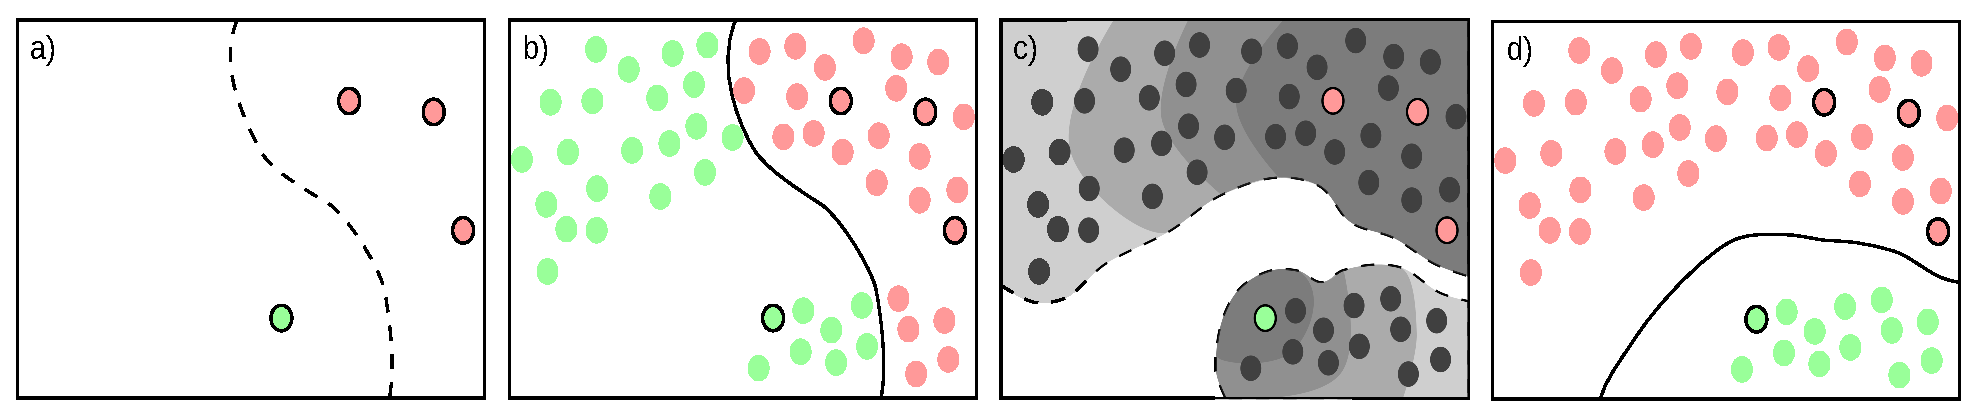
\includegraphics[width=\textwidth]{fig/semivssuperv.eps}
	\caption[Aprendizaje semi-supervisado vs supervisado]{Ejemplo de clasificación con aprendizaje supervisado (a-b) y con aprendizaje semi-supervisado (c-d).}
	\label{fig:semivssuperv}
\end{figure}

\section{Predicción automática de microARN}

En los últimos años, la biología molecular demostró un importante avance en distintas áreas de la investigación. Esta disciplina científica
estudia la estructura, función y composición de las moléculas biológicamente importantes y se relaciona fuertemente con otras áreas como la
genética y la bioquímica. En la actualidad se invierte un gran esfuerzo en estudiar las interacciones entre los numerosos sistemas de las células,
incluyendo las interacciones entre los diferentes tipos de ácido desoxirribonucleico (ADN), ácido ribonucleico (ARN) y los procesos de síntesis de
proteínas, y también cómo estas interacciones son reguladas. Los avances en este campo permiten la generación de una gran cantidad de información
que requiere el uso de herramientas de cálculo altamente especializadas para el análisis. En este contexto, la bioinformática ha tomado un papel muy
importante ya que aporta herramientas que posibilitan la explotación de estos datos.

Un problema abierto en Bioinformática desde hace más de una década es el de la predicción automática de microARNs (miARNs). Los miARNs son una clase de
pequeñas moléculas ($\sim$21 nucleótidos) monocatenarias de ácido desoxirribonucleico no codificante que regulan la expresión de otros genes. Se
encuentran presentes tanto en animales como en plantas y su importancia en procesos biológicos clave ha sido ampliamente documentada
\citep{rosenzvit2013microrna}. Los miARNs están implicados, por ejemplo, en la evolución del cáncer (sea como inhibidores o promotores de éste)
\citep{yu2015microrna}, en procesos de infección viral \citep{lecellier2005}. Además, identificar los microARNs de ciertas especies tiene aplicaciones
directas, como puede en plantas ser la mejora de cultivos \citep{liu2010new} o, en animales,  el desarrollo de nuevas vacunas y antibióticos
\citep{tsetsarkin2017synergistic}. Estas pequeñas moléculas normalmente se transcriben a partir de secuencias primarias de mayor tamaño, llamadas
pri-miARNs. Durante la biogénesis, las secuencias precursoras se pliegan sobre sí mismas formando una estructura secundaria tipo tallo-horquilla como se
puede ver en la Figura~\ref{fig:mirna}. Luego son separadas de la secuencia principal y trasladadas fuera del núcleo. En este paso, la estructura toma el
nombre de precursora del miARN o pre-miARN. Finalmente el miARN es liberado del precursor para tomar un papel activo en la regulación de la expresión de los
genes.

\begin{figure}[tpb]
	\centering
	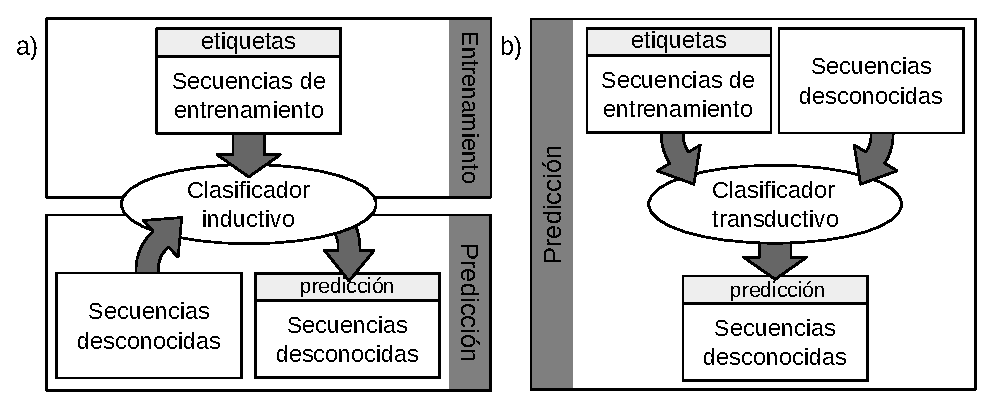
\includegraphics[width=\textwidth]{fig/paradigmas.eps}
	\caption[Aprendizaje inductivo vs. transductivo]{Aprendizaje inductivo y transductivo. a) Esquema tradicional inductivo con dos etapas separadas; b)
	Esquema transductivo con sólo una etapa.}
	\label{fig:schemes}
\end{figure}

En la última década, se utilizaron numerosos enfoques experimentales y computacionales para identificar nuevos miARNs. Los métodos experimentales que se han
usado tradicionalmente como el clonado directo son capaces de detectar sólo miARNs que se expresan de forma abundante \citep{kleftogiannis2013where}. Los
últimos avances en secuenciación permiten un alto nivel de cobertura, mitigando estos efectos \citep{an2013mirdeep}. Sin embargo, aquellos que se expresan en
ciertas etapas de una especie, o en tejidos específicos, pueden no ser detectados. Por otro lado, el desarrollo y posterior análisis de los modelos
computacionales entrenados para reconocer miARNs puede brindar pistas que permitan caracterizar mejor estas moléculas y su biogénesis. Los enfoques
computacionales utilizados para la clasificación de secuencais candidatas a miARN pueden dividirse en dos grupos: métodos por homología y métodos de aprendizaje
automático. Los primeros se basan en la conservación de miARNs entre especies estrechamente relacionadas y, por lo tanto, no pueden usarse para miARNs que son
específicos de una especie \citep{ng2007novo}. Los métodos de aprendizaje automático utilizan un enfoque diferente, que consiste en extraer primero
características de pre-miARNs conocidos, de secuencias que se utilizarán como ejemplos negativos y de las secuencias desconocidas que se desea clasificar.
Después se utilizan las características de las secuencias conocidas (tanto positivas como negativas) para entrenar un clasificador de forma supervisada, para
finalmente aplicarlo a las secuencias no conocidas y obtener una predicción \citep{kleftogiannis2013where}. Las características que pueden usarse para
representar secuencias de ARN han sido ampliamente estudiadas \citep{Lopes2014}. Además, muchos algoritmos de aprendizaje supervisado han sido aplicados a este
problema: máquinas de soporte vectorial, modelos ocultos de Markov y ensambles de clasificadores, entre otros \citep{kleftogiannis2013where}. Sin embargo
todavía existen muchos problemas abiertos en la predicción de pre-miARNs con técnicas de aprendizaje maquinal \citep{stegmayer2018predicting}.

La gran mayoría de los métodos de predicción del estado del arte toman como entrada secuencias con estructura secundaria tipo tallo-horquilla y se encargan
luego de extraer características, entrenar un clasificador y hacer predicciones. Si bien este primer paso generalmente es ignorado, es fundamental para lograr
buenos resultados en las etapas posteriores. No sólo es importante lograr capturar todas las secuencias con estructura secundaria tipo tallo horquilla del
genoma, sino que también es fundamental que estas secuencias se corten en los lugares correctos. Si un pre-miARN se corta erróneamente con una longitud mayor
o menor a la real, las características calculadas pueden variar mucho y generar resultados erróneos durante la etapa de predicción. Actualmente, la única
herramienta disponible para esta tarea \citep{durbin1999einverted} no aprovecha los últimos avances en cuanto a la estimación de estructuras secundarias, por
lo que el número de secuencias que detecta es bajo y muchos pre-miARN se pierden durante esta temprana etapa. Además, no se tiene en cuenta el contexto de la
secuencia para detectar dónde son los mejores puntos de corte. Las características utilizadas en la predicción de pre-miARN son muy sensibles a pequeñas
diferencias en el corte, por lo que elegir el punto óptimo es crucial para obtener buenos resultados en la clasificación.

Por otro lado, durante la última década se ha desarrollado una gran cantidad de características específicamente para el problema de predicción de
microARN, que se pueden extraer tanto de las secuencias o sus estructuras secundarias. Se han publicado muchas herramientas para calcular algunas de estas
características, pero estas están codificadas en diferentes lenguajes de programación y tienen diferentes modos de acceso (web, línea de comandos, etc.).
Además, varias de estas herramientas son software propietario y el código fuente no está disponible \footnote{http://www.insybio.com/pages/ncrnaseq}. Estas
cuestiones dificultan en gran medida el uso de muchas de estas características.

\begin{figure}[t]
	\centering
	\includegraphics[width=\textwidth]{fig/mirna.pdf}
	\caption[Estructura secundaria de un pre-miARN]{Estructura secundaria de un pre-miARN humano. En rojo se puede ver resaltado el miARN hsa-let-7e.}
	\label{fig:mirna}
\end{figure}

Por último, la etapa de predicción o clasificación de secuencias como posibles candidatos a pre-miARN aún presenta importantes dificultades que no han sido
resueltas satisfactoriamente. En primer lugar, aunque el número de secuencias no pre-miARN que se pueden encontrar en cualquier genoma es grande, los ejemplos
negativos que se utilicen deben ser representativos de la gran variedad de secuencias no pre-miARN. Un estudio \citep{wei2014improved} analizó la
importancia de los ejemplos negativos utilizados y cómo esto limita el rendimiento de los clasificadores. En la mayoría de los casos, los conjuntos negativos
que se usan para ajustar los modelos de clasificación se definen principalmente con secuencias tomadas de regiones de codificación de proteínas, ARNm u otras
regiones donde es poco probable encontrar miARN \citep{peace2015framework, tempel2015mirboost}. Nada puede asegurar que estas secuencias sean buenos
representantes de todas las posibles secuencias no pre-miARN, o que estén lo suficientemente cerca de los límites de la verdadera clase de pre-miARN. Por ejemplo,
si el poder de predicción de un clasificador se prueba en un conjunto de datos que tiene pre-miARNs y ncARNs, lo que realmente se está midiendo es la capacidad
de diferenciar entre estos dos tipos de secuencia, pero el clasificador podría no descartar correctamente otras secuencias no pre-miARN. Ningún método ha
informado tasas de error teniendo en cuenta este punto crucial. Para abordar este problema, algunos métodos utilizan secuencias tomadas de posiciones aleatorias
de un genoma como ejemplos negativos \citep{wenyuan2013training, gudys2013huntmi}. Sin embargo, en este caso, nada puede garantizar que un pre-miARN no conocido
se utilice erróneamente como un ejemplo negativo. En ambas estrategias de construcción de conjuntos de ejemplos negativos, no se puede garantizar que los
ejemplos sean representativos de toda la clase negativa; y, lo que es peor, algunos de ellos podrían ser falsos negativos. Otra característica de este problema
que dificulta la aplicación simple de técnicas de aprendizaje maquinal es el hecho de que el número de ejemplos positivos es muy bajo en cualquier genoma, por
lo cual este constituye un problema con muy alto desbalance entre clases. Este problema es aún peor en especies no modelo, donde la cantidad de secuencias
anotadas es menor. Una alternativa puede ser utilizar pre-miARNs de especies cercanas como ejemplos positivos, pero recientemente se ha demostrado
\citep{lopes2016automatic} que el problema de predicción de pre-miARNs es muy dependiente de la especie, por lo que esta estrategia puede afectar el desempeño
de las técnicas de predicción. Por otro lado, la gran variedad de secuencias que se pueden utilizar como ejemplos negativos y el bajo número de ejemplos
positivos obliga a entrenar clasificadores con un desbalance muy grande entre el número de secuencias positivas y las potencialmente negativas. Esto presenta
una dificultad adicional ya que está demostrado que las  técnicas estándar de aprendizaje maquinal son muy sensibles al desbalance de clases
\citep{guo2008class}.

